% =====================================================================================================
% MMIBC figure setup.  \input this ONCE in the preamble of the paper (or of a standalone wrapper).
% The fragments (fig_architecture.tex, fig_algorithm.tex) are drawn for a 12.2 cm text width
% (Springer LNCS / MICCAI).  For another width wrap the fragment, e.g.
%     \resizebox{\linewidth}{!}{% Architecture of MMIBC v2 with the corrections to the rejected submission marked.  Cn = row of tab_corrections.tex.
% Drawn for a 12.2 cm text width: six columns of 1.88 cm with 0.18 cm gaps.
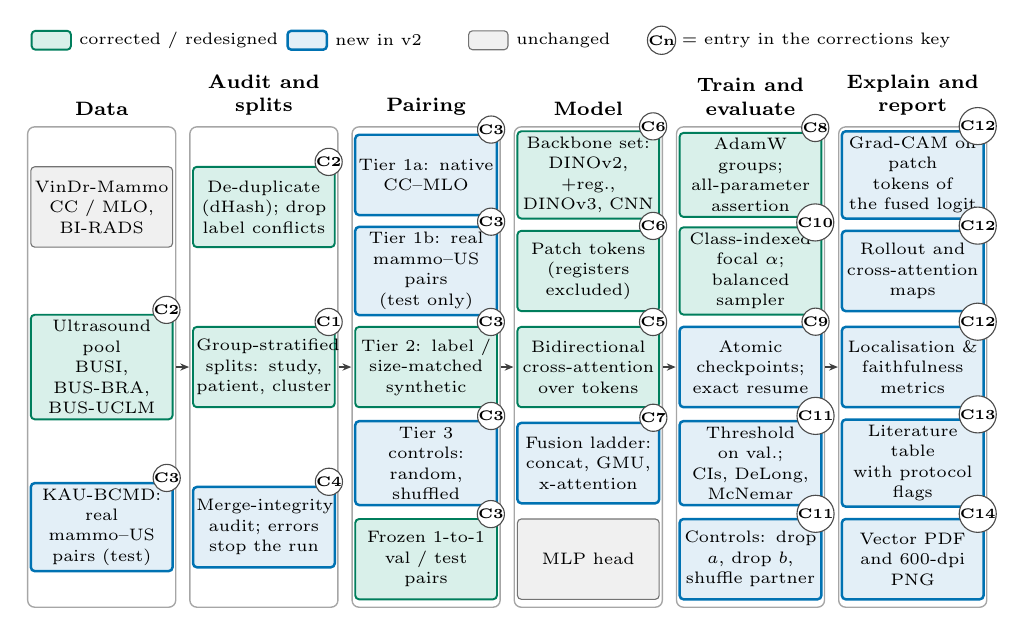
\begin{tikzpicture}[x=1cm,y=1cm]
  \useasboundingbox (0,-0.02) rectangle (12.2,7.36);   % pin the box to the 12.2 cm text width
  % ---- legend ---------------------------------------------------------------------------------------
  \node[corr, minimum width=0.5cm, minimum height=0.24cm] at (0.3,7.2) {};
  \node[anchor=west, font=\mmfs, inner sep=0pt] at (0.65,7.2) {corrected / redesigned};
  \node[newb, minimum width=0.5cm, minimum height=0.24cm] at (3.55,7.2) {};
  \node[anchor=west, font=\mmfs, inner sep=0pt] at (3.9,7.2) {new in v2};
  \node[same, minimum width=0.5cm, minimum height=0.24cm] at (5.85,7.2) {};
  \node[anchor=west, font=\mmfs, inner sep=0pt] at (6.2,7.2) {unchanged};
  \node[mmbadge] at (8.05,7.2) {Cn};
  \node[anchor=west, font=\mmfs, inner sep=0pt] at (8.3,7.2) {= entry in the corrections key};

  % ---- column frames and titles ---------------------------------------------------------------------
  \foreach \i/\t in {0/Data, 1/{Audit and\\splits}, 2/Pairing, 3/Model, 4/{Train and\\evaluate}, 5/{Explain and\\report}}{
    \draw[mmcol] ({\i*2.06},0) rectangle ++(1.88,6.1);
    \node[mmhead, anchor=south] at ({\i*2.06+0.94},6.2) {\t};
  }
  \foreach \i in {0,...,4}
    \draw[mmarr] ({\i*2.06+1.88+0.01},3.05) -- ({(\i+1)*2.06-0.01},3.05);

  % ---- column 1: data -------------------------------------------------------------------------------
  \mmblock{d1}{same}{0.94}{5.083}{1.80cm}{1.02cm}{VinDr-Mammo\\CC / MLO,\\BI-RADS}{}
  \mmblock{d2}{corr}{0.94}{3.05 }{1.80cm}{1.02cm}{Ultrasound pool\\BUSI, BUS-BRA,\\BUS-UCLM}{C2}
  \mmblock{d3}{newb}{0.94}{1.017}{1.80cm}{1.02cm}{KAU-BCMD:\\real mammo--US\\pairs (test)}{C3}

  % ---- column 2: audit and splits -------------------------------------------------------------------
  \mmblock{a1}{corr}{3.0}{5.083}{1.80cm}{1.02cm}{De-duplicate\\(dHash); drop\\label conflicts}{C2}
  \mmblock{a2}{corr}{3.0}{3.05 }{1.80cm}{1.02cm}{Group-stratified\\splits: study,\\patient, cluster}{C1}
  \mmblock{a3}{newb}{3.0}{1.017}{1.80cm}{1.02cm}{Merge-integrity\\audit; errors\\stop the run}{C4}

  % ---- column 3: pairing ----------------------------------------------------------------------------
  \mmblock{p1}{newb}{5.06}{5.49}{1.80cm}{1.02cm}{Tier 1a: native\\CC--MLO}{C3}
  \mmblock{p2}{newb}{5.06}{4.27}{1.80cm}{1.02cm}{Tier 1b: real\\mammo--US pairs\\(test only)}{C3}
  \mmblock{p3}{corr}{5.06}{3.05}{1.80cm}{1.02cm}{Tier 2: label /\\size-matched\\synthetic}{C3}
  \mmblock{p4}{newb}{5.06}{1.83}{1.80cm}{1.02cm}{Tier 3 controls:\\random,\\shuffled}{C3}
  \mmblock{p5}{corr}{5.06}{0.61}{1.80cm}{1.02cm}{Frozen 1-to-1\\val / test\\pairs}{C3}

  % ---- column 4: model ------------------------------------------------------------------------------
  \mmblock{m1}{corr}{7.12}{5.49}{1.80cm}{1.02cm}{Backbone set:\\DINOv2, +reg.,\\DINOv3, CNN}{C6}
  \mmblock{m2}{corr}{7.12}{4.27}{1.80cm}{1.02cm}{Patch tokens\\(registers\\excluded)}{C6}
  \mmblock{m3}{corr}{7.12}{3.05}{1.80cm}{1.02cm}{Bidirectional\\cross-attention\\over tokens}{C5}
  \mmblock{m4}{newb}{7.12}{1.83}{1.80cm}{1.02cm}{Fusion ladder:\\concat, GMU,\\x-attention}{C7}
  \mmblock{m5}{same}{7.12}{0.61}{1.80cm}{1.02cm}{MLP head}{}

  % ---- column 5: train and evaluate -----------------------------------------------------------------
  \mmblock{t1}{corr}{9.18}{5.49}{1.80cm}{1.02cm}{AdamW groups;\\all-parameter\\assertion}{C8}
  \mmblock{t2}{corr}{9.18}{4.27}{1.80cm}{1.02cm}{Class-indexed\\focal $\alpha$;\\balanced sampler}{C10}
  \mmblock{t3}{newb}{9.18}{3.05}{1.80cm}{1.02cm}{Atomic\\checkpoints;\\exact resume}{C9}
  \mmblock{t4}{newb}{9.18}{1.83}{1.80cm}{1.02cm}{Threshold on val.;\\CIs, DeLong,\\McNemar}{C11}
  \mmblock{t5}{newb}{9.18}{0.61}{1.80cm}{1.02cm}{Controls: drop\\$a$, drop $b$,\\shuffle partner}{C11}

  % ---- column 6: explain and report -----------------------------------------------------------------
  \mmblock{x1}{newb}{11.24}{5.49}{1.80cm}{1.02cm}{Grad-CAM on\\patch tokens of\\the fused logit}{C12}
  \mmblock{x2}{newb}{11.24}{4.27}{1.80cm}{1.02cm}{Rollout and\\cross-attention\\maps}{C12}
  \mmblock{x3}{newb}{11.24}{3.05}{1.80cm}{1.02cm}{Localisation \&\\faithfulness\\metrics}{C12}
  \mmblock{x4}{newb}{11.24}{1.83}{1.80cm}{1.02cm}{Literature table\\with protocol\\flags}{C13}
  \mmblock{x5}{newb}{11.24}{0.61}{1.80cm}{1.02cm}{Vector PDF\\and 600-dpi\\PNG}{C14}
\end{tikzpicture}%
}
% Colours are the Okabe-Ito colour-blind-safe palette; status is also encoded by line weight and fill
% luminance so the figures survive greyscale printing.
% =====================================================================================================
\usepackage{amsmath,amssymb,booktabs,array}
\usepackage{tikz}
\usetikzlibrary{arrows.meta,calc,fit,backgrounds,shapes.geometric}

\definecolor{mmG}{HTML}{009E73}   % corrected / redesigned
\definecolor{mmB}{HTML}{0072B2}   % new in v2
\definecolor{mmO}{HTML}{D55E00}   % gradient / back-propagation
\definecolor{mmY}{HTML}{E69F00}   % decision

\providecommand*{\mmfs}{\fontsize{6.4}{7.4}\selectfont}
\providecommand*{\mmfnh}{\mmfs\hyphenpenalty=10000 \exhyphenpenalty=10000 }
\providecommand*{\mmfh}{\fontsize{7.4}{8.6}\selectfont\bfseries}

\tikzset{
  mmblk/.style  = {rounded corners=1.4pt, align=center, inner xsep=1.2pt, inner ysep=2pt, font=\mmfnh},
  corr/.style   = {mmblk, draw=mmG!80!black, fill=mmG!15, line width=0.7pt},
  newb/.style   = {mmblk, draw=mmB, fill=mmB!11, line width=0.9pt},
  same/.style   = {mmblk, draw=black!55, fill=black!6, line width=0.4pt},
  mmarr/.style  = {-{Stealth[length=3.2pt,width=2.6pt]}, line width=0.6pt, draw=black!75},
  mmgrad/.style = {-{Stealth[length=3.2pt,width=2.6pt]}, line width=0.75pt, draw=mmO, dash pattern=on 2.4pt off 1.6pt},
  mmbadge/.style= {circle, draw=black!70, fill=white, line width=0.4pt, inner sep=0pt, minimum size=7.4pt,
                   font=\fontsize{4.9}{5}\selectfont\bfseries, text=black},
  mmcol/.style  = {rounded corners=2.5pt, draw=black!35, line width=0.5pt},
  mmhead/.style = {font=\mmfh, align=center, inner sep=1pt},
  mmnote/.style = {font=\fontsize{6}{7}\selectfont\itshape, align=left, inner sep=0pt},
}

% \mmbadges{node}{C4,C1}: correction-number badges along the top-right edge of a node; the FIRST item is the right-most
% (so list them in descending order to read C1 C4 from left to right)
\newcommand{\mmbadges}[2]{%
  \foreach \mmb [count=\mmi from 0] in {#2}{%
    \node[mmbadge] at ($(#1.north east)+(-0.09cm-\mmi*0.40cm,0.05cm)$) {\mmb};}}

% \mmblock{name}{style}{x}{y}{width}{height}{text}{badges}
\newcommand{\mmblock}[8]{%
  \node[#2, minimum width=#5, minimum height=#6, text width=#5-2.4pt] (#1) at (#3,#4) {#7};%
  \ifx\relax#8\relax\else\mmbadges{#1}{#8}\fi}
